\section{Evaluation}
An important driving factor for this project and the application developed was a system of evaluation at all levels of development. To that end, the student employed a
number of techniques and phases to convert feedback into actionable input that would then influence how the project progressed. Each of those techniques is covered in detail in the following subsections.

\subsection{Development Testing Process} \label{devtest}
Under PXP, the refactor branch was adapted to also serve as a final testing stop before the student pushed code to production (See \ref{devflow}). Automated testing was considered as mentioned in the Design section (See \ref{automatedtests}) but was found to not be suitable for this project.

Instead, refactoring was done manually on the refactoring branch based on visual inspection for rendering artifacts. To help with this process, a python command line tool was written to generate a wide range of datasets for edge case testing. The datasets and python tool are all attached in appendix \ref{A4} but some notable datasets are as follows:

\begin{itemize}
    \item DataCube - This is a data set that creates a 10x10x10 Cube of data points. If the application renders correctly, this dataset would fill every visible space (with a grid pattern) at the initial zoom and slice position. (See Figure \ref{fig:satur})
    \item Terrain Data - This is a Stress test dataset consisting of perlin noise generated terrain coordinates in a 30x30x30 sized chunk of 27000 points. It is a test for not only performance but also ability to handle data points with decimal values. (See Figure \ref{fig:nocolpick})
\end{itemize}

Other testing datasets were also manually created using excel:
\begin{itemize}
    \item Minimal Data - A single data point at 1, 1, 1. Minimal test to make sure uploading files works and renders correctly
    \item Hidden Data - 1 Point - A navigation and zoom test, single point at -25, 25, -25
    \item Negative Data - 100 Points all with one or more negative component. Made to test negative data
\end{itemize}

These datasets also served to provide a wide range of example data for user testers to use in addition to datasets created specifically for user testing:
\begin{itemize}
    \item Coffee Shop Stats - 60 Points - For testing 4 dimension analysis
    \item Nutritional Information of Popular Cereals (Single Serving) - 100 Points - A dataset to test if users could notice patterns in 3D data using the application (See Figure \ref{fig:cereal})
    \item Secret Structure Data - 40,000 Points - Performance and navigation test, renders a Pyramid in negative y space, generated with Python (See Figure \ref{fig:pyramid})
    \item Sine Wave - 200 Points - Tests specific point identification and general structure analysis
\end{itemize}

\begin{figure}[hbt!]
    \centering
    \begin{subfigure}
        \centering
        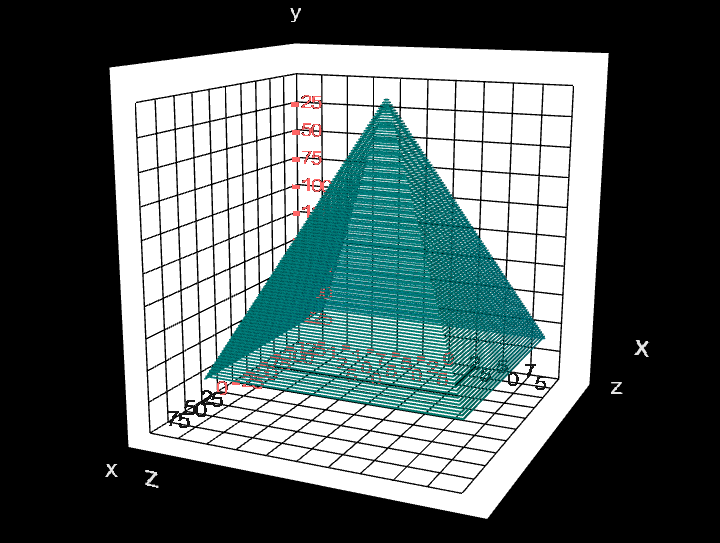
\includegraphics[width=1\columnwidth]{author-files/figures/pyramid.PNG}
        \caption{Secret Structure Data, Forms a Pyramid}
        \label{fig:pyramid}
    \end{subfigure}
    \hfill
    \begin{subfigure}
        \centering
        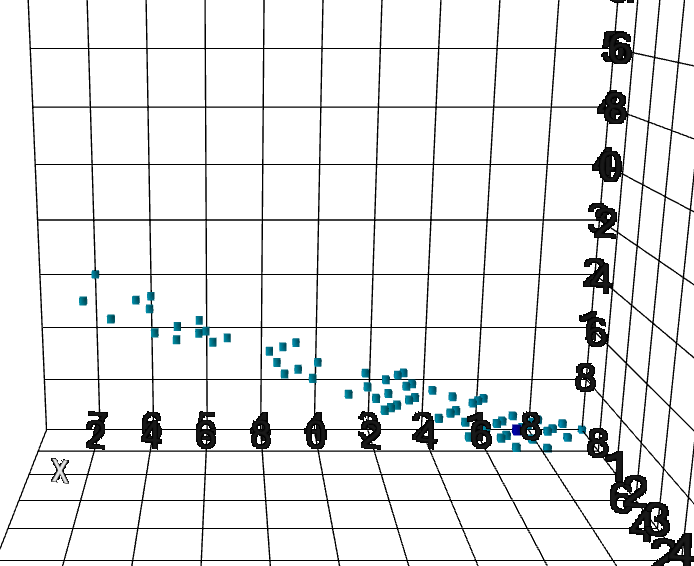
\includegraphics[width=1\columnwidth]{author-files/figures/cerealdata.PNG}
        \caption{Nutritional Information of Popular Cereals (Single Serving)}
        \label{fig:cereal}
    \end{subfigure}
\end{figure}

\subsection{User Testing} \label{usertest1}
User testing was an important step in gathering requirements and paving the way for further development beyond the most basic, fundamental requirements. In total, 2 User testing phases were ran. The first one after the completion of the MVP feature set post Sprint 5 and the second one after the completion of the further additions feature set and user testing 1 feature set post sprint 8.

The process for these two phases revolved around an anonymous questionnaire with data collected as per the prepared ethics documentation for honours students.
To support the testing process, the student created a simple static webpage to act as a central source for all links to the application, the questionnaire, testing data and ethics documentation that guided a tester through the entire process. Having this page really simplified testing as the student would only need to share a single link which self-contained everything needed. The page itself and HTML source is available to view in the appendix \ref{A5}.

The questionnaires themselves asked a tester to download a specific dataset and use the application to identify some factor or knowledge placed in the data by the student. The datasets were also designed in such a way that the questions could best be solved if the tester used some specific controls, or understood some aspect of the graph that the test focused on. This was also followed by the testers personal thoughts on a variety of questions concerning usability and how they went about solving the problems set out.

This allowed the student to construct a critical understanding of how real users used the application to solve typical problems the application was designed in mind with. Were users able to get the correct answer? What controls did they use? Did they use the controls as the student expected? Though it should be mentioned that the results likely aren't fully representative of the demographic tested due to the limited number of testers. Of which, a majority were computing students. This likely shifted results for usability specifically. Though ideally, testing tried to represent college students who were likely to work with data and all Adults in general.

The responses collected were then analyzed and turned into user stories to be developed, with the two testing phases each forming the User Testing 1 feature set and User Testing 2 Feature set respectively. The following give specific detail of each phase and the analysis performed on user stories. All questionnaire questions and responses are available for viewing at Appendix \ref{A6}.

\subsubsection{User Testing 1 - Starting February 17th} \label{usertestanalysis}
This was setup and ran right after sprint 5 was complete. The focus for this testing phase was to identify what controls were still missing to help users do real work using the application. The questionnaire was created to that end and user testing began. The user testing was then concluded a week later with 5 total responses. In general responses were positive, though there were some trending limitations and gripes across testers:

\begin{itemize}
    \item Controls were good but a bit bare-bones. Most suggestions recorded were quality of life additions to the UI.
    \item Identifying specific node values was the least popular task across testers. With the overall NPS (Net Promoter Score) being at a -25, the lowest recorded value in the test.
\end{itemize}

These points were interesting because otherwise, most testers rated ease of control usability quite high- At a NPS score of +40. The overall feel was that the user controls that were there were good but not enough to fully explore the data as was asked.

The answers given formed user stories which were analyzed and prioritized using MoSCoW and the Workload Estimate system previously used for the MVP feature set. All of theses stories formed the User Testing 1 feature set which was given a 1 month total development time (to be completed on the 1st of April). The feature set was then divided among 4 sprints as follows:

\begin{itemize}
    \item Sprint 5 - See Stories on Table \ref{sprint5}
    \item Sprint 6 - See Stories on Table \ref{sprint6}
    \item Sprint 7 - See Stories on Table \ref{sprint7}
    \item Sprint 8 - See Stories on Table \ref{sprint8}
    \item Some User Stories though, were chosen to not be developed, they are mentioned here (See Table \ref{UT1})
\end{itemize}

Some notable analysis notes on user stories follows:

\begin{itemize}
    \item Story 57 (See Table \ref{UT1}) was pinpointed to Apple Devices, which would not render the chart correctly. It is unknown what the issue exactly is but it is likely something to do with how Apple supports WebGL \cite{khronosgroup_2022_webgl} (See 'Metal' in 2.2.3).
    \item Story 56 (See Table \ref{UT1}) was created after one tester mentioned poor performance using the Opera browser. Nothing specific towards this claim was found so this may have been a problem on the testers device.
    \item Story 50 (See Table \ref{UT1}) was created on popular demand to have automatically rendering trendlines. This would have required a math library to generate a best fit line for the data which would be rendered. This task was not assigned to a sprint due to limited time but could be a good future addition.
    \item Story 51 (See Table \ref{UT1}) was proposed to solve the same point identification as picking which was done in favor of this as it was more popular (and helpful in the Students opinion).
    \item Story 49 (See Table \ref{UT1}) was created after a tester asked if they could search thorough the data. This is an interesting use case that implies the suitability of having a database backend for running queries on data as a possibly useful feature. See Databases in Future work, \ref{futurework}
    \item Story 55 (See Table \ref{UT1}) was created when a tester asked for data points to not intersect. This was found to be too difficult to cover edge cases for as a balance between visibility and non-interaction had to be found for any possible values of points- This story was abandoned in favor of keeping the user themselves in control of sizing
\end{itemize}

In summary, this user test identified a number of UI problems and opportunities to expand how users can better interact and view the data.

\subsubsection{User Testing 2 - Starting March 30th} \label{usertestanalysis2}
This was setup and ran right after sprint 8 was complete. The focus for this testing phase was to see if the new controls made tasks easier to do and what users thought of the new 4th dimension representation. The questionnaire was once again created and the testing concluded on the 21st of April with 8 responses. In general, responses were positive and trended towards being more positive than during the last user test- previous testers (The questionnaire asked to answer some questions if they previously tested, See \ref{A6}) rated the application as much better with an overall NPS score of +100. Further key points were as follows:

\begin{itemize}
    \item Identifying specific node values rose from an overall NPS of -25 to +57, with multiple testers mentioning that they used the new hover system to identify points. This implies that the new picking system for selecting points successfully solved the arguably biggest issue identified during the last user test (See Identifying specific node values in \ref{usertestanalysis}).
    \item The new zoom was unanimously favored over the old one by repeating testers- and positively viewed by new testers.
    \item The Data Management had a positive impact on user experience. Most testers used it in their tasks and found it as a helpful addition to the overall graph view. Though many testers mentioned bugs in how the table was presented and with some selectors. This was found to be likely a result of state bugs specifically and a cause of uncovered edge cases.
    \item The Help tab was much less popular than the other tabs but still was rated as useful by the few testers that used it.
    \item Clarity of data points was the biggest issue mentioned by multiple people. Bad clarity was mentioned in general with specific descriptions being "grittiness", "flickering" and "dots on numbers".
    \item The 4th dimension had mixed results, most testers did not understand it's use and opted to use only the 3D graphing functionality. Those that did use it mentioned further difficultly with how to use it.
\end{itemize}

The overall consensus was that usability and design has improved dramatically over the first user testing phase and most issues mentioned dealt with bugs rather than problems with using the application. As for the 4th dimension, it's addition to the application had not been done very well. Further design and modification will be required to better communicate it's use and simplify operation for users.

The answers given were once again analyzed and prioritized using MoSCoW and the Workload Estimate system previously used. All of theses stories formed the User Testing 2 feature set which would make a good start for future development.
The user stories are all compiled here (See Table \ref{UT2})

Some notable analysis notes on user stories are as follows:
\begin{itemize}
    \item Story 87 was been pinpointed to be a performance issue when labels are updated, such as when the graph slice is moved using the movement controls (See \ref{spr3} for more details) This confirms that the decision done to prepare all labels before rendering was the right way to go as otherwise labels would flicker constantly every frame (See glyph rendering rework in \ref{spr3}). Though the performance is still not suitable, the model class would have to be looked at for opportunities to increase performance.
    \item Story 88 refers to user tester mentioning dotted dots on numbers. The student believes that this may be some issue with how the fragment shader for text clips the texture. Further optimization and research is needed.
    \item Story 85 mentions inaccuracy in picking. This could be caused by the off-screen buffer texture somehow becoming out of tune with the size of the actual screen (Resizing browser tab) but further research is needed to confirm this and identify any other edge cases.
    \item Story 83 may be a repeated issue with the Opera browser but is likely also the result of more demanding datasets given to be tested (See Secret Structure Data in \ref{devtest})
\end{itemize}

In summary, this testing phase has made a number of important points very clear for the application. The functionality that is there is very successful and fixes almost all problems previously faced by by testers during the first test phase. Except for the 4th dimension functionality, the application implements all needed controls and functionality to be a successful analysis tools for the questions poised to testers. The main drawbacks though are a number of bugs within the UI and within the renderer. The bugs within the UI almost all stem from incorrect management of state edge cases and is the first time a precedent is set to justify bringing in outside tools for the direct sake of the user experience quality. Otherwise, when this problem was last visited this important precedent was missing (See the refactoring discussion during sprint 5, \ref{s5}).

\subsection{Further Improvements Feature Set}
The further improvement feature sets were created to encompass all created tasks that did not directly link back to a suggestion or issue mentioned by testers. These tasks instead focused on what the student thought would be valuable additions based on their research (Similar to how the MVP feature set was created, see \ref{reqgat}) and analysis of user testing trends. 2 of these feature sets were created in total with each being in tandem with the creation of the User testing feature sets (See \ref{usertest1}). These feature sets were considered by the student as an important part of overall evaluation and acted as a culmination of further gathered requirements in the context of user testing.

Further Improvements Feature Set 1 tasks were allocated across the 4 sprints after sprint 4, to be completed in 1 month (On the 1st of April). The set consisted of 6 total tasks and focused on general ideas that the student had to improve the application. Those can be seen per sprint as follows:

\begin{itemize}
    \item Sprint 6 - See Stories on Table \ref{sprint6-2}
    \item Sprint 7 - See Stories on Table \ref{sprint7-2}
\end{itemize}

Further Improvements Feature Set 2 would make a great starting point for future development. This set consists of 7 total tasks and focuses on ways to fix the applications current problems. Those tasks can be seen on Table \ref{FI2}.